\documentclass[a4paper]{article}

\usepackage[text={16cm, 25cm}, left=2.8cm, top=1.8cm]{geometry}
\usepackage[T1]{fontenc}
\usepackage[utf8x]{inputenc}
\usepackage[linguistics]{forest}
\usepackage[hidelinks,unicode]{hyperref}
\usepackage[czech]{babel}
\usepackage{color}
\usepackage{parskip}
\usepackage{algorithm2e}

\usepackage{tikz}
\def\checkmark{\tikz\fill[green,scale=0.4](0,.35) -- (.25,0) -- (1,.7) -- (.25,.15) -- cycle;} 

\usepackage{multicol}

\usepackage{amsmath}
\usepackage{amsthm}

\theoremstyle{definition}
\newtheorem{definition}{Definice}

\newcounter{rulenum}
\setcounter{rulenum}{1}
\newcommand{\nter}[1]{\textcolor{blue}{\,#1\,}}
\newcommand{\ter}[1]{\textbf{\textcolor{red}{\,#1\,}}}
\newcommand{\precter}[1]{\textcolor{orange}{\,#1\,}}
\newcommand{\grule}[2]{{\small\arabic{rulenum}. \stepcounter{rulenum} \nter{#1} $\to$ #2}\\}
\newcommand{\drule}[2]{\checkmark \grule{#1}{#2}}


\title{Gramatická pravidla jazyka IFJ21}

\begin{document}
	
\begin{titlepage}
	\begin{center}
	
\includegraphics[width=\linewidth]{inc/FIT_logo.pdf}\\
	\vspace{\stretch{0.2}}
	{\Huge
		Implementace překladače imperativního jazyka IFJ21\\[0.5em] Tým 005, varianta I.
	}\\
	\vspace{\stretch{0.8}}
	\begin{minipage}{0.6\linewidth}
		\begin{center}
		\Large
		\begin{tabular}{l c r}
			\textbf{Tadeáš Vintrlík} & \texttt{xvintr04} & $25\%$ \\
			Kryštof Albrecht & \texttt{xalbre05} & $25\%$ \\
			Josef Škorpík & \texttt{xskorp07} & $25\%$ \\
			Jakub Kozubek & \texttt{xkozub07} & $25\%$ \\
		\end{tabular}
		\end{center}
	\end{minipage}
	\end{center}
	\vfill
	\today
\end{titlepage}

\newpage

\tableofcontents

\newpage

\section{Spolupráce v týmu}

Při práci na projektu jsme využívali metodu párového programování. Díky pravidelným setkáním, osobně i přes Discord, měl každý přehled o dění v projektu a nebylo nutné využívat nástroje, jako je Trello.

Pro verzování zdrojových kódu projektu jsme využívali GitHub.


\subsection{Rozdělení práce}



\subsubsection{Tadeáš Vintrlík}

\begin{itemize}
	\item Tabulka symbolů

	\item Abstraktní datové typy - seznam, zásobník, AVL stromy

	\item Testy pro ADT a syntaktický analyzátor
	
	\item Generování kódu

	\item Sémantické kontroly
	
	\item Precedenční analyzátor
\end{itemize}

\subsubsection{Kryštof Albrecht}

\begin{itemize}
	\item Syntaktický analyzátor shora-dolů

	\item Lexikální analyzátor
	
	\item LL-gramatika
\end{itemize}

\subsubsection{Josef Škorpík}

\begin{itemize}
	\item Automat pro lexikální analýzu

	\item Lexikální analyzátor
	
	\item Syntaktický analyzátor shora-dolů
\end{itemize}

\subsubsection{Jakub Kozubek}

\begin{itemize}
	\item Generování kódu
	
	\item ADT dynamický řetězec

	\item Testy pro lexikální analyzátor

	\item Precedenční tabulka
\end{itemize}

\newpage

\section{Návrh překladače}



\subsection{Lexikální analyzátor}

Lexikální analyzátor je implementován v souboru \texttt{scanner.c}.


\subsubsection{Diagram konečného automatu}

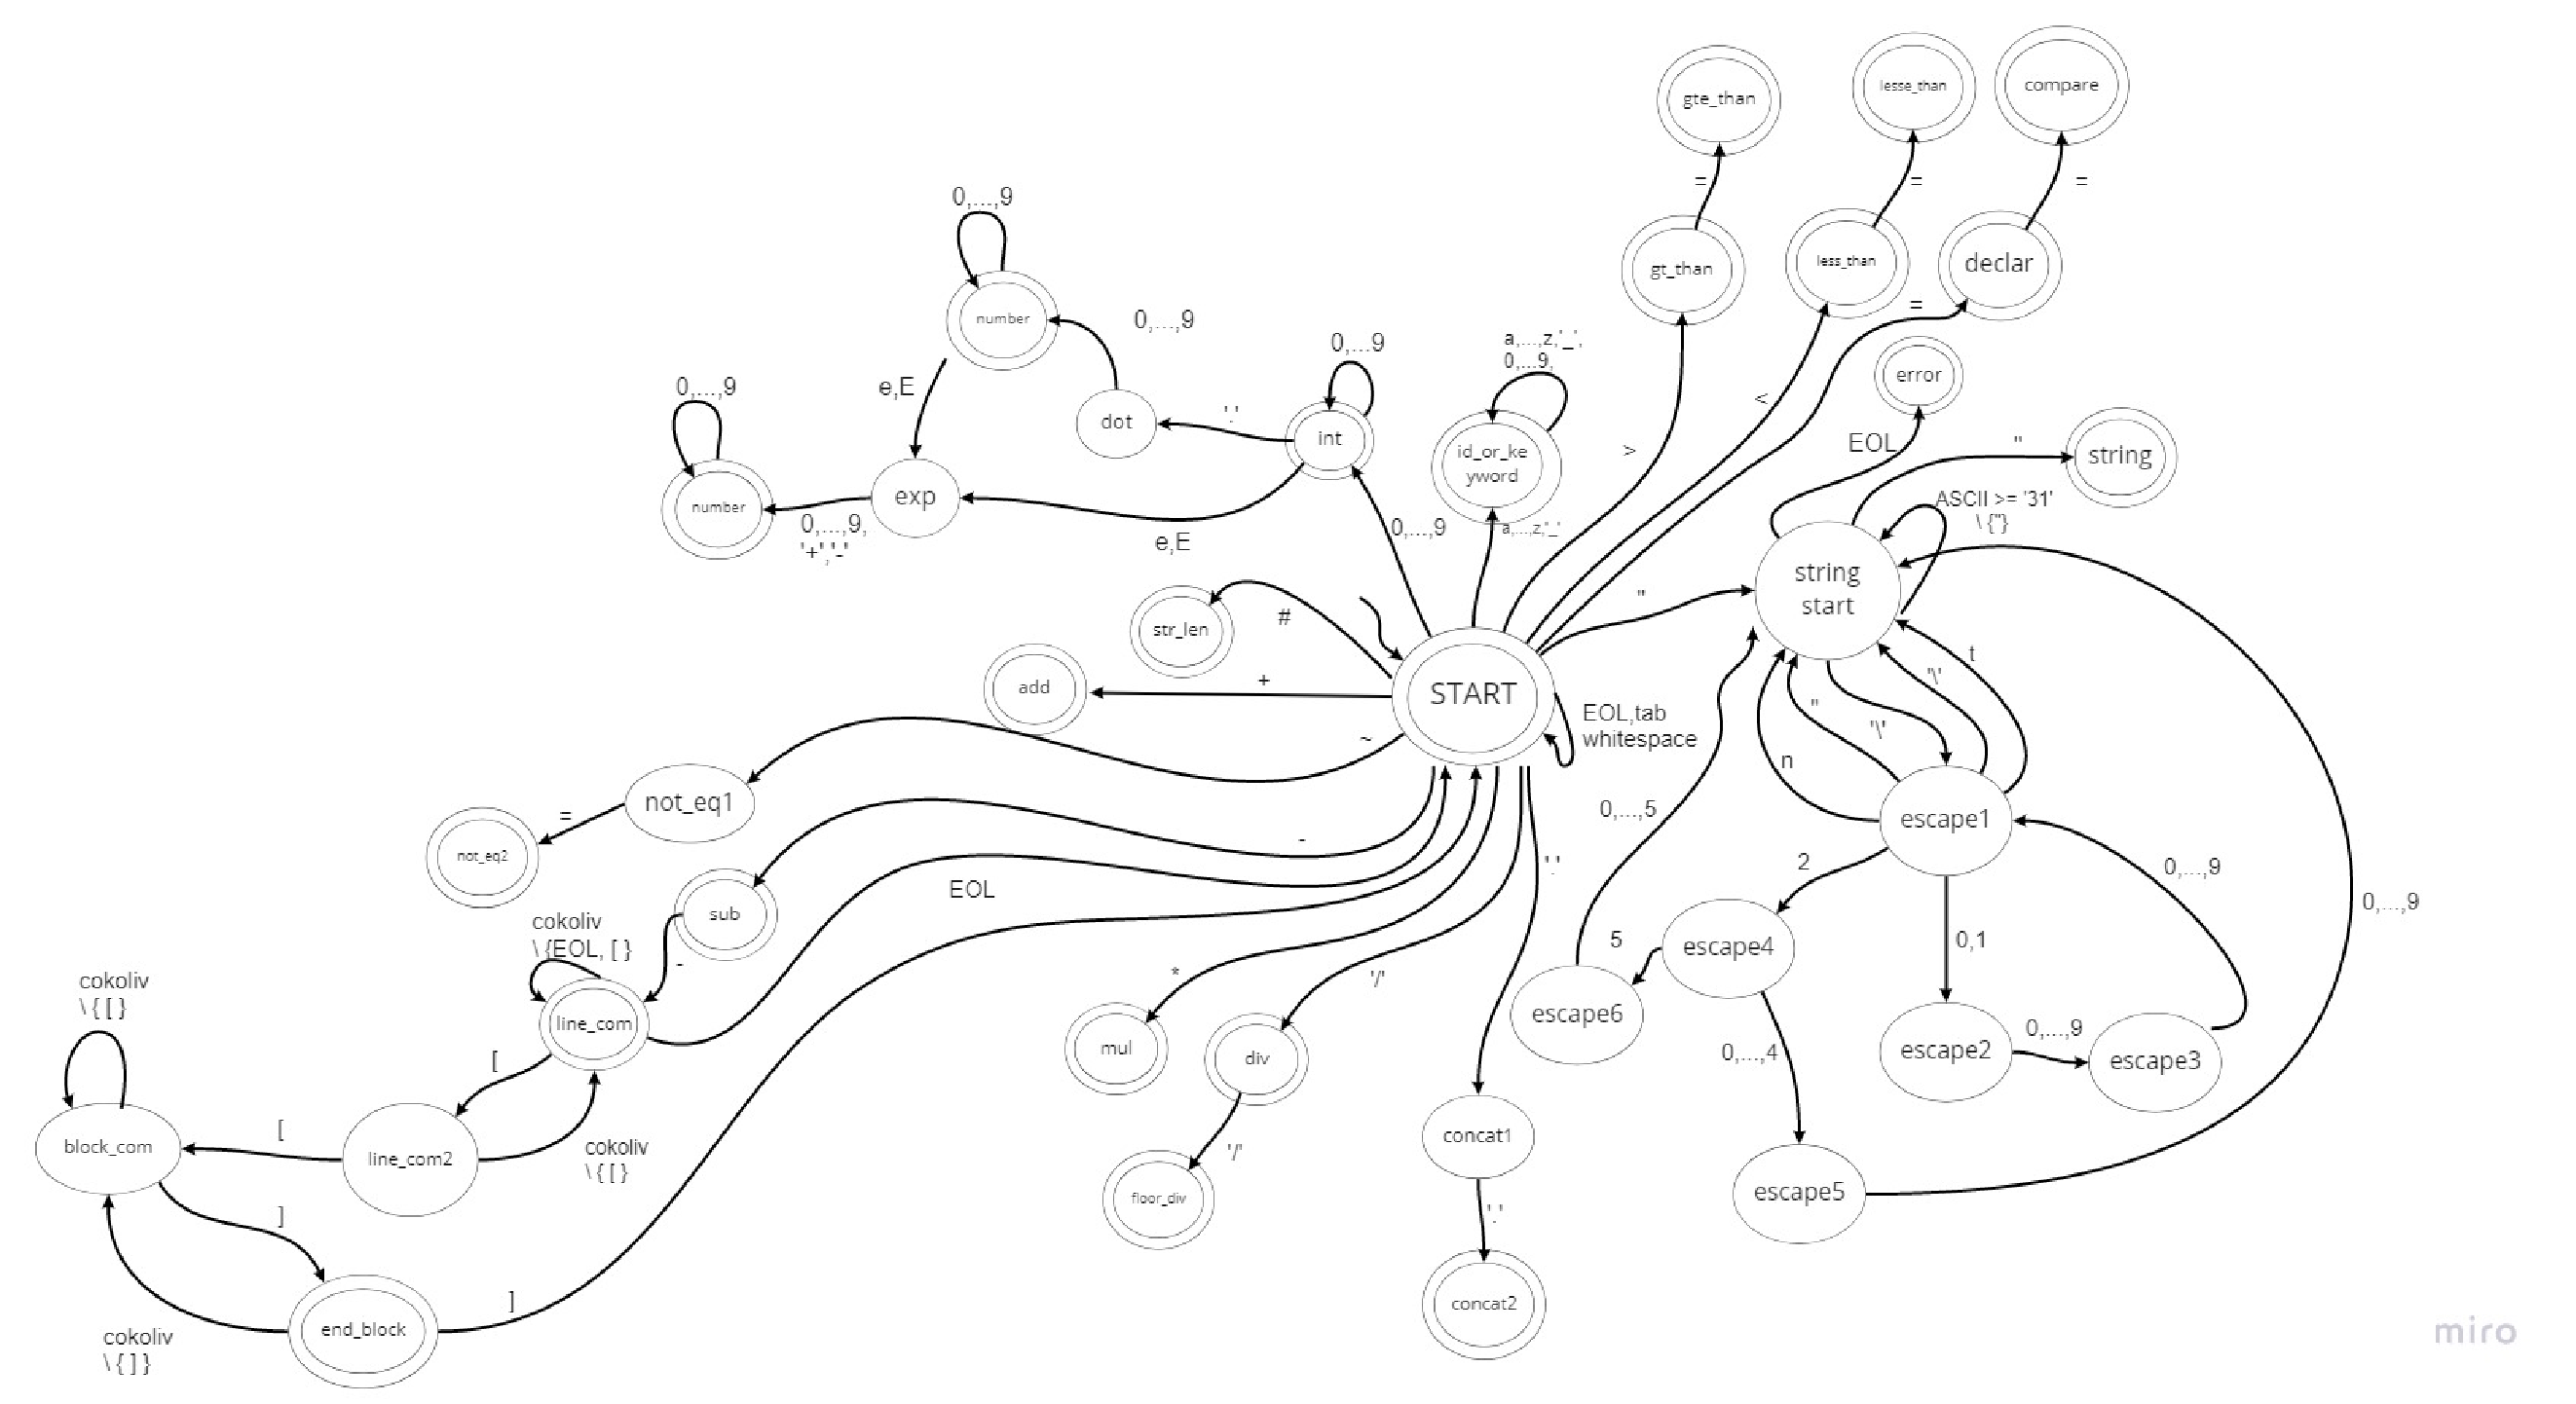
\includegraphics[width=\linewidth]{./inc/automaton.pdf}

\subsubsection{Reprezentace tokenů a symbolů}

Datová struktura reprezentující tokeny je implementována v souboru \texttt{token\_stack.h}.

Struktura je využívána nejen lexikálním analyzátorem, ale také tabulkou symbolů a během sémantických kontrol. Z tohoto důvodu obsahuje informace nejen o typu lexémy a atribut, ale také o datovém typu.

Při deklaraci proměnných a funkcí se jednoduše vezme token od scanneru, přiřadí se mu sémantické informace a je uložen do tabulky symbolů.

Umožňuje to také například přiřazovat datový typ literálům teprve vráceným lexikálním analyzátorem, což usnadňuje analýzu výrazů.


\subsubsection{Funkce \texttt{unget\_token(T\_token*)}}\label{sec_unget_token}

Jelikož se syntaktický analyzátor nemůže u některých konstrukcí jazyka IFJ21 jednoznačně rozhodnout podle jednoho tokenu, implementuje scanner funkci pro vracení tokenů zpět.

Tato funkce natlačí token na zásobník tokenů [\ref{tstack}], ze kterého potom bere funkce \texttt{get\_next\_token()} tokeny přednostně.

\subsection{Syntaktický analyzátor}

Syntaktický analyzátor je implementován v souboru \texttt{parser.c}.

Jako metodu pro analýzu shora-dolů jsme zvolili rekurzivní sestup. Pojmenování funkcí v kódu je vždy ve tvaru \texttt{rule\_\nter{NTER}}, kde \texttt{\nter{NTER}} je jeden z neterminálů uvedených na levé straně gramatických pravidel [\ref{sec_grammar}].

\newpage

\subsubsection{LL-gramatika}\label{sec_grammar}

	\grule{PROG}{\ter{require} \ter{lit\_string} \nter{CODE}}
	\grule{CODE}{\ter{$\epsilon$}}
	\grule{CODE}{\nter{TOP\_ELEM} \nter{CODE}}
	\grule{TOP\_ELEM}{\nter{CALL}}
	\grule{TOP\_ELEM}{\nter{DECL}}
	\grule{TOP\_ELEM}{\nter{DEF}}
	\grule{DECL}{\ter{global} \ter{id} \ter{:} \ter{function} \ter{(}\nter{TYPE\_LIST}\ter{)} \nter{RET\_LIST}}
	\grule{DEF}{\ter{function} \ter{id} \ter{(} \nter{PARAM\_LIST} \ter{)} \nter{RET\_LIST} \nter{BODY} \ter{end}}
	\grule{CALL}{\ter{id} \ter{(} \nter{ARG\_LIST} \ter{)}}
	\grule{RET\_LIST}{\ter{:} \nter{TYPE} \nter{NEXT\_TYPE}}
	\grule{RET\_LIST}{\ter{$\epsilon$}}
	\grule{TYPE\_LIST}{\nter{TYPE} \nter{NEXT\_TYPE}}
	\grule{TYPE\_LIST}{\ter{$\epsilon$}}
	\grule{NEXT\_TYPE}{\ter{,} \nter{TYPE} \nter{NEXT\_TYPE}}
	\grule{NEXT\_TYPE}{\ter{$\epsilon$}}
	\grule{TYPE}{\ter{nil}}
	\grule{TYPE}{\ter{integer}}
	\grule{TYPE}{\ter{number}}
	\grule{TYPE}{\ter{string}}
	\grule{ARG\_LIST}{\nter{ARG} \nter{NEXT\_ARG}}
	\grule{ARG\_LIST}{\ter{$\epsilon$}}
	\grule{NEXT\_ARG}{\ter{,} \nter{ARG} \nter{NEXT\_ARG}}
	\grule{NEXT\_ARG}{\ter{$\epsilon$}}
	\grule{ARG}{\ter{id}}
	\grule{ARG}{\ter{lit\_number}}
	\grule{ARG}{\ter{lit\_int}}
	\grule{ARG}{\ter{lit\_string}}
	\grule{ARG}{\ter{nil}}
	\grule{PARAM\_LIST}{\nter{PARAM} \nter{NEXT\_PARAM}}
	\grule{PARAM\_LIST}{\ter{$\epsilon$}}
	\grule{NEXT\_PARAM}{\ter{,} \nter{PARAM} \nter{NEXT\_PARAM}}
	\grule{NEXT\_PARAM}{\ter{$\epsilon$}}
	\grule{PARAM}{\ter{id} \ter{:} \nter{TYPE}}
	\grule{BODY}{\ter{$\epsilon$}}
	\grule{BODY}{\nter{STAT\_LIST}}
	\grule{STAT\_LIST}{\nter{VAR\_DECL} \nter{STAT\_LIST}}
	\grule{STAT\_LIST}{\nter{IF\_ELSE} \nter{STAT\_LIST}}
	\grule{STAT\_LIST}{\nter{WHILE} \nter{STAT\_LIST}}
	\grule{STAT\_LIST}{\ter{return} \precter{EXPR\_LIST}}
	\grule{VAR\_DECL}{\ter{local} \ter{id} \ter{:} \nter{TYPE} \ter{=} \precter{EXPR}}
	\grule{IF\_ELSE}{\ter{if} \nter{EXPR} \ter{then} \nter{BODY} \ter{else} \nter{BODY} \ter{end}}
	\grule{WHILE}{\ter{while} \nter{EXPR} \ter{do} \nter{BODY} \ter{end}}

\subsubsection{LL-tabulka}

\begin{center}
	\scalebox{0.4}{
\begin{tabular}{| l || c | c | c | c | c | c | c | c | c | c | c | c | c | c | c | c | c | c | c | c | c | c | c | c | c |}
	                   & \ter{(} & \ter{)} & \ter{:} & \ter{,} & \ter{=} & \ter{do} & \ter{else} & \ter{end} & \ter{function} & \ter{global} & \ter{id} & \ter{if} & \ter{integer} & \ter{lit\_int} & \ter{lit\_number} & \ter{lit\_string} & \ter{local} & \ter{nil} & \ter{number} & \ter{require} & \ter{return} & \ter{string} & \ter{then} & \ter{while} & \ter{\$} \\\hline
	\nter{PROG}        &         &         &         &         &         &          &            &           &                &              &          &          &               &                &                   &                   &             &           &              & 1             &              &              &            &             & \\\hline
	\nter{CODE}        &         &         &         &         &         &          &            &           &    3           &         3    &  3       &          &               &                &                   &                   &             &           &              &               &              &              &            &             & 2\\\hline
	\nter{TOP\_ELEM}   &         &         &         &         &         &          &            &           &         6      &      5       &     4    &          &               &                &                   &                   &             &           &              &               &              &              &            &             & \\\hline
	\nter{DECL}        &         &         &         &         &         &          &            &           &                & 7            &          &          &               &                &                   &                   &             &           &              &               &              &              &            &             & \\\hline
	\nter{DEF}         &         &         &         &         &         &          &            &           & 8              &              &          &          &               &                &                   &                   &             &           &              &               &              &              &            &             & \\\hline
	\nter{CALL}        &         &         &         &         &         &          &            &           &                &              & 9        &          &               &                &                   &                   &             &           &              &               &              &              &            &             & \\\hline
	\nter{RET\_LIST}   &         &         &    10   &         &         &          &            &      11   &      11        &      11      &      11  &    11    &               &                &                   &                   &      11     &           &              &               &      11      &              &            &      11     & 11 \\\hline
	\nter{TYPE\_LIST}  &         &    11   &         &         &         &          &            &           &                &              &          &          &      12       &                &                   &                   &             &      12   & 12           &               &              &      12      &            &             & \\\hline
	\nter{NEXT\_TYPE}  &         &     15  &         &     14  &         &          &            &      15   &      15        &      15      &     15   &      15  &               &                &                   &                   &      15     &           &              &               &      15      &              &            &      15     & 15 \\\hline
	\nter{TYPE}        &         &         &         &         &         &          &            &           &                &              &          &          &      17       &                &                   &                   &             &      16   &      18      &               &              &     19       &            &             & \\\hline
	\nter{ARG\_LIST}   &         &    21   &         &         &         &          &      21    &      21   &                &              &      20  &          &               &      20        & 20                &  20               &             &      20   &              &               &              &              &            &             & \\\hline
	\nter{NEXT\_ARG}   &         &   23    &         &     22  &         &          &      23    &      23   &                &              &          &          &               &                &                   &                   &             &           &              &               &              &              &            &             & \\\hline
	\nter{ARG}         &         &         &         &         &         &          &            &           &                &              &     24   &          &               &         26     &      25           &           27      &             &      28   &              &               &              &              &            &             & \\\hline
	\nter{PARAM\_LIST} &         &    30   &         &         &         &          &            &           &                &              &      29  &          &               &                &                   &                   &             &           &              &               &              &              &            &             & \\\hline
	\nter{NEXT\_PARAM} &         &  32     &         &    31   &         &          &            &           &                &              &          &          &               &                &                   &                   &             &           &              &               &              &              &            &             & \\\hline
	\nter{PARAM}       &         &         &         &         &         &          &            &           &                &              &     33   &          &               &                &                   &                   &             &           &              &               &              &              &            &             & \\\hline
	\nter{BODY}        &         &         &         &         &         &          &    34      &     34    &                &              &          &    35    &               &                &                   &                   &      35     &           &              &               &    35        &              &            &      35     & \\\hline
	\nter{STAT\_LIST}  &         &         &         &         &         &          &            &           &                &              &          &    37    &               &                &                   &                   &      36     &           &              &               &      39      &              &            &      38     & \\\hline
	\nter{VAR\_DECL}   &         &         &         &         &         &          &            &           &                &              &          &          &               &                &                   &                   &      40     &           &              &               &              &              &            &             & \\\hline
	\nter{IF\_ELSE}    &         &         &         &         &         &          &            &           &                &              &          &   41     &               &                &                   &                   &             &           &              &               &              &              &            &             & \\\hline
	\nter{WHILE}       &         &         &         &         &         &          &            &           &                &              &          &          &               &                &                   &                   &             &           &              &               &              &              &            &    42       & \\

\end{tabular}
}
\end{center}

\subsubsection{Konstrukce nepokryté LL-gramatikou} %TODO

V jazyce IFJ21 jsou dvě konstrukce, které porušují LL(1) -- jsou to příkazy \emph{přiřazení} a \emph{volání funkce bez přiřazení}:

\begin{enumerate}
	\item \texttt{\ter{id}\ter{(}\nter{ARG\_LIST}\ter{)}}

	\item \texttt{\ter{id}\ter{,}\ter{id}\ter{,}\dots \ter{=} \precter{EXPR}\ter{,}\precter{EXPR}\ter{,}\dots}

	\item \texttt{\ter{id}\ter{,}\ter{id}\ter{,}\dots \ter{=} \ter{id} \ter{(} \nter{ARG\_LIST} \ter{)}}
\end{enumerate}

U pravidla \nter{STAT\_LIST} by tedy nastala kolize v množině \emph{First}.

Rozhodnutí, který případ ve zpracovaném zdrojovém kódu nastal, probíhá získáním tokenu za identifikátorem.

Jestliže tento token je \ter{(}, oba tokeny jsou vráceny scanneru [\ref{sec_unget_token}] a pokračuje se pravidlem \texttt{rule\_\nter{CALL}}. V opačném případě se předpokládá přiřazení -- sesbírají se identifikátory na levé straně (\texttt{left\_side\_function}) a předají se funkci zpracovávající přiřazení (\texttt{right\_side\_function}). 

Zda na pravé straně je volání či seznam výrazů se určuje téměř identickým způsobem.

\subsection{Precedenční analýza}

Analyzátor výrazů je implementován v souboru \texttt{exp\_parser.c}.

Jelikož v jazyce IFJ21 nejsou ukončovače výrazů, precedenční analyzátor rozlišuje následující případy:

\begin{enumerate}
	\item Doposud přečtený výraz je platný a byl přečten nečekaný token -- výraz je označen za platný, nečekaný token vrácen a řízení předáno top-down parseru

	\item Přečtený výraz je zatím prázdný a hned první token je nečekaný -- výraz je označen za prázdný, nečekaný token vrácen a řízení předáno top-down parseru (ten nepřítomnost výrazu může buď schválit, či zamítnout)
	
	\item Přijatý výraz není platný a byl přečten nečekaný token -- syntaktická chyba
\end{enumerate}

\subsubsection{Precedenční tabulka}

\begin{center}
\scalebox{0.8}{
\begin{tabular}{l || c | c | c | c | c | c | c | c | c |}
                                  & \ter{\#} & \ter{*},\ter{/},\ter{//} & \ter{+},\ter{-} & \ter{..} & \ter{<},\ter{~=},\ \dots & \ter{(} & \ter{)} & \ter{id} & \ter{\$} \\\hline
     \ter{\#}                     & >        & >                        & >               & >        & >                        & <       & >       & <        & > \\\hline
     \ter{*},\ter{/},\ter{//}     & <        & >                        & >               & >        & >                        & <       & >       & <        & > \\\hline
     \ter{+},\ter{-}              & <        & <                        & >               & >        & >                        & <       & >       & <        & > \\\hline
     \ter{..}                     & <        & <                        & <               & <        & >                        & <       & >       & <        & > \\\hline
     \ter{<},\ter{~=},\ \dots     & <        & <                        & <               & <        & X                        & <       & >       & <        & > \\\hline
     \ter{(}                      & <        & <                        & <               & <        & <                        & <       & =       & <        & X \\\hline
     \ter{)}                      & X        & >                        & >               & >        & >                        & X       & >       & X        & > \\\hline
     \ter{id}                     & X        & >                        & >               & >        & >                        & <       & >       & X        & > \\\hline
     \ter{\$}                     & <        & <                        & <               & <        & <                        & <       & X       & <        & X \\\hline
\end{tabular}
}
\end{center}



\subsection{Sémantické kontroly}\label{sec_semantics}

Sémantické kontroly jsou implementovány v souboru \texttt{semantics.c}.

\subsection{Generování kódu}

Vypisování cílového kódu na standardní výstup probíhá průběžně voláním funkcí implementovaných v souboru \texttt{code\_gen.c}. 

\subsubsection{Řešení kolizí v návěštích u podmíněných příkazů a funkcí}

Všechna návěští začínají pomlčkou, kterou nelze použít v IFJ21 v identifikátorech.

Návěští podmíněných příkazů jsou číslována podle čítače, který při každém použití příkazu \texttt{if} či \texttt{while} inkrementuje.

Návěští vestavěných funkcí začínají pomlčkou (tak jako u podmíněných příkazů), zatímco návěští uživatelských funkcí začínají procentem. %TODO TAKTO TO NEFUNGUJE ZATIM


\subsubsection{Parametry a návratové hodnoty funkcí}

Před zavoláním funkce je vytvořen Temporary Frame, do kterého jsou přiřazeny potřebné parametry (\texttt{TF@\%pN}), včetně případného přetypování.

Funkce po zavolání provede \texttt{PUSHFRAME} a přesune získané parametry do patřičných lokálních proměnných.

Návratové hodnoty se ukládají do \texttt{LF@\%retvalN}. Po dokončení funkce se provede \texttt{POPFRAME} a volající z Temporary Frame přesune návratové hodnoty do lokálních proměnných (u volání s přiřazením).

\subsubsection{Vyhodnocování výrazů}

Kód pro vyhodnocování výrazů je generován přímo při precedenční analýze při redukci. K vyhodnocování je v IFJcode21 využíván datový zásobník. 

Při přiřazování jsou nejdříve všechny výrazy vyhodnoceny (tím pádem zůstanou na datovém zásobníku) a poté pomocí \texttt{POPS LF@\dots} přiřazeny.

\subsection{Tabulka symbolů}\label{sec_symtable}
Podle zvolené varianty zadání jsme měli implementovat Tabulku symbolů pomocí binárních vyhledávacích stromů.
Pro implementaci bylo použito hned několik abstraktních datových struktur.

\subsubsection{AVL Strom}
Jako základní datová struktura tabulky byl použit binární vyhledávací strom, konkrétně jejich samovyvažující varianta dvou Ruských matematiků Adeľson-Velského a Landise. Základ zdrojového kódu byl přebrán z druhého projektu z předmětu Algoritmy a doplněn, aby odpovídal specifikaci AVL stromů. Implementace se nachází v souboru \texttt{avl.c}.

\subsubsection{Jednosměrně svázaný seznam}
Jednosměrně svázaný seznam byla další datová struktura použitá nejen v tabulce symbolů, ale v rámci celého projektu
a sloužila jako základ pro abstraktní datový typ zásobník\label{tstack}. Implementace se nachází v souborech \texttt{sll.c} a \texttt{token\_stack.c}.
\\ \\
V tabulce symbolů jsou tyto dvě struktury použity dohromady, kdy celá tabulka symbolů má následující rozložení:
\begin{enumerate}
    \item Globální AVL strom použitý pro funkce.
    \item Zásobník AVL stromů pro lokální proměnné.
\end{enumerate}

Zásobník zde byl zvolen pro jeho vhodnost při simulování rámců platnosti.


\end{document}
